%Example of use of Time Domain Astrophysics latex class
\documentclass{tda}

\usepackage{booktabs}
\usepackage{hyperref}
\usepackage[font=footnotesize,labelfont=bf]{caption}
\usepackage{subcaption}
\usepackage{afterpage}

%define the page header/title info
\course{Time Domain Astrophysics --- 2020/21 --- Data Exercise} %DON'T EDIT ME!

\begin{document}

\section{Introduction \& Aims}
The primary aim of this exercise is to analyse the evolution of a classical nova using photometry and spectroscopy. Using these two tools, we wish to classify the nova in terms of its light-curve and speed class. Combining the information, we eventually try to estimate the distance to this nova. The methods, results and analysis are discussed for photometry in section \ref{sec:photometry} and for spectroscopy in section \ref{sec:spectroscopy}. Discussions and conclusions are also presented alongside the presentation of related results in the same section \ref{sec:everything}, followed by a list of references.

\section{Methods, Results \& Analysis} \label{sec:everything}

	\subsection{Photometry} \label{sec:photometry}

	Photometry of the nova is performed using the GAIA software which is a part of Starlink suite of software applications. The images when viewed in software initially provide little or no information with few white dots on a dark background. To help with extracting information from the images, the \emph{auto cut, colour map, intensity map} and \emph{colour bar} features are used according to the requirements. The \emph{auto cut} feature, which is sufficient in most cases, varies the data limits on brightest and faintest object in the image. A value of 98-99.5\% is optimum for most images. The other three features are used to vary the number, scale and palette of image colours, which may help in providing a better visualization. 

	In order to perform the photometry, the basic necessity is to first successfully locate the nova in the provided series of 18 SDSS \textit{r'}-band photographic images obtained using Liverpool Telescope. For this, the images are compared and the object whose brightness varies (eventually fades) over time is identified at position \((1055,978)\) on every image grid, which corresponds to right ascention and declination of the object at roughly \(\alpha = 00:44:41.05\) and \(\delta = 40:08:36.00\), respectively. 

	The format of the images file is called \emph{FITS} - Flexible Image Transport System. It consists of two sections -- \emph{image header} followed by \emph{image data}. The header provides a lot of information about the image, a few of which, like the DATE-OBS (date/time of observation), MJD (modified Julian date), EXPTIME (exposure time), GAIN (photoelectrons per data unit) and AIRMASS (relative optical path length through atmosphere) are noted, for further use in performing photometry. The EXPTIME for initial sixteen images (phot\(\_\)00.fits -- phot\(\_\)15.fits) is 120 seconds, while for the final two images (phot\(\_\)16.fits and phot\(\_\)17.fits) the value is 300 seconds. The value of GAIN for each image is noted to be 1.62 photoelectrons per data unit.

	For each image, point spread function (PSF) of the nova is observed, and the its span along x-axis in units of number of pixels is noted and summarized in table \ref{table:aperture_and_span}. The value for image phot\(\_\)11.fits could not be obtained given that the nova in the image could not be located with enough confidence possibly due to poor photometric conditions. It can be seen that, in general, the span is seen to roughly decrease over time and remains roughly constant in the final images, where exposure time is increased. This trend can be attributed to possible two effects -- change in viewed psf of nova and variation in sky (background) brightness. Our estimates of the same are also biased by the value of differing values of auto cut used in different images. Therefore, decrease in span can be attributed most prominently to reducing PSF of the nova.

	\begin{table} [h]
	\centering
	\begin{tabular} {l r r}
		\toprule
		\textbf{file} & \textbf{x-axis span} & \textbf{aperture} \\
		\midrule
		phot\(\_\)00.fits & 1049–1061 & 7.0 \\
		phot\(\_\)01.fits & 1049–1061 & 6.5 \\
		phot\(\_\)02.fits & 1049–1061 & 5.5 \\
		phot\(\_\)03.fits & 1050–1061 & 5.4 \\
		phot\(\_\)04.fits & 1052–1058 & 4.9 \\
		phot\(\_\)05.fits & 1053–1058 & 4.9 \\
		phot\(\_\)06.fits & 1052–1058 & 8.0 \\
		phot\(\_\)07.fits & 1053–1058 & 4.4 \\
		phot\(\_\)08.fits & 1050–1060 & 7.5 \\
		phot\(\_\)09.fits & 1053–1058 & 4.6 \\
		phot\(\_\)10.fits & 1053–1058 & 3.1 \\
		phot\(\_\)11.fits & --		  & 4.4 \\
		phot\(\_\)12.fits & 1053–1057 & 3.6 \\
		phot\(\_\)13.fits & 1054–1057 & 2.5 \\
		phot\(\_\)14.fits & 1054–1057 & 2.3 \\
		phot\(\_\)15.fits & 1054–1056 & 4.2 \\
		phot\(\_\)16.fits & 1053–1056 & 3.3 \\
		phot\(\_\)17.fits & 1054–1056 & 2.9 \\
		\bottomrule
	\end{tabular}
	\caption{The span of PSF of the nova across x-axis, in units of pixels range, and the size (semi-major-axis) of optimal aperture, in units of number of pixels, calculated for different photometric image files.}
	\label{table:aperture_and_span}
\end{table}


	To perform the approximate photometry, the \emph{Aperture Photometry in magnitudes} option is used first. For this, we use a frame zero point of 0 magnitudes and input the values of exposure time and gain for the image being analysed. Image of a faint object captured over long exposure time may be brighter than the image of a bright object captured over smaller exposure time. Similarly, high gain would require more photons per data unit. Therefore, our perception of bright and faint objects may vary from one image to another with varying exposure times and gains. Hence, it is important to account for both of these parameters for each image. 

	Once these values are entered, a circular aperture is defined over the nova with surrounding annulus used for estimating background noise. A very small aperture would lead to loss of signal by discarding useful signal. A large aperture would include a lot of noise. Hence in both cases, signal to noise ratio is decreased, although in different manners. An optimal aperture considers all the signal while discarding maximum possible noise. The value of estimated background noise from the annulus is subtracted from the value obtained from aperture (which contains both signal from nova and noise) to obtain true signal. Consequently, the most optimal aperture is the one with maximum signal as well as highest signal-to-noise ratio.

	Upon performing photometry for different combinations of aperture and annulus radii, it is observed that the errors are not statistical, but instead depend upon the radius of the aperture used. Both small and large apertures are inefficient and an optimum aperture lies in between that range.

	To estimate an optimal aperture size for an image, \emph{Aperture Photometry using data counts} option is used. For a range of values of aperture sizes, the values of mean counts, error in counts and signal-to-noise ratios (SNR) are noted. For image phot\(\_\)00.fits, the variation in SNR with aperture size is shown in figure \ref{fig:SNR_aperture}. It should be noted that the value of aperture size calculated for an image should be retained across all measurements performed using that image. This is to make sure that we account for the same ratio of light received from each object in the image and therefore, consistent relative values of brightness are obtained. 

	\begin{figure}
		\begin{subfigure}{.49\textwidth}
			\centering
			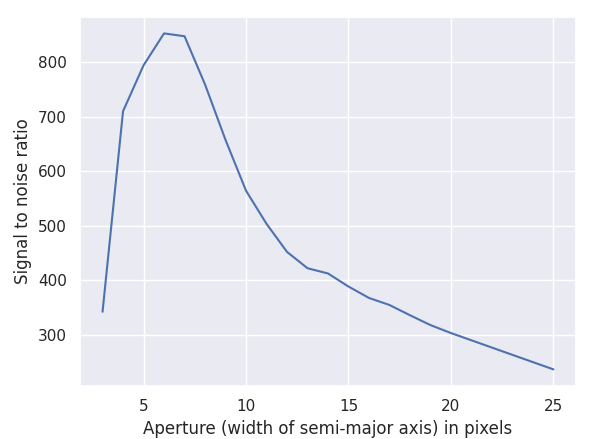
\includegraphics[width=\linewidth]{../codes/plots/optimal_aperture_phot_00.png}
			\caption{Variation of signal-to-noise ratio with aperture size for the nova in first photometric image file phot\(\_\)00.fits. For each entry, inner and outer radii of annulus are \(r_a=1.5\) pixels and \(r_b=2.0\) pixels respectively.}
			\label{fig:SNR_aperture}
		\end{subfigure}%
		\hfill
		\begin{subfigure}{.49\textwidth}
			\centering
			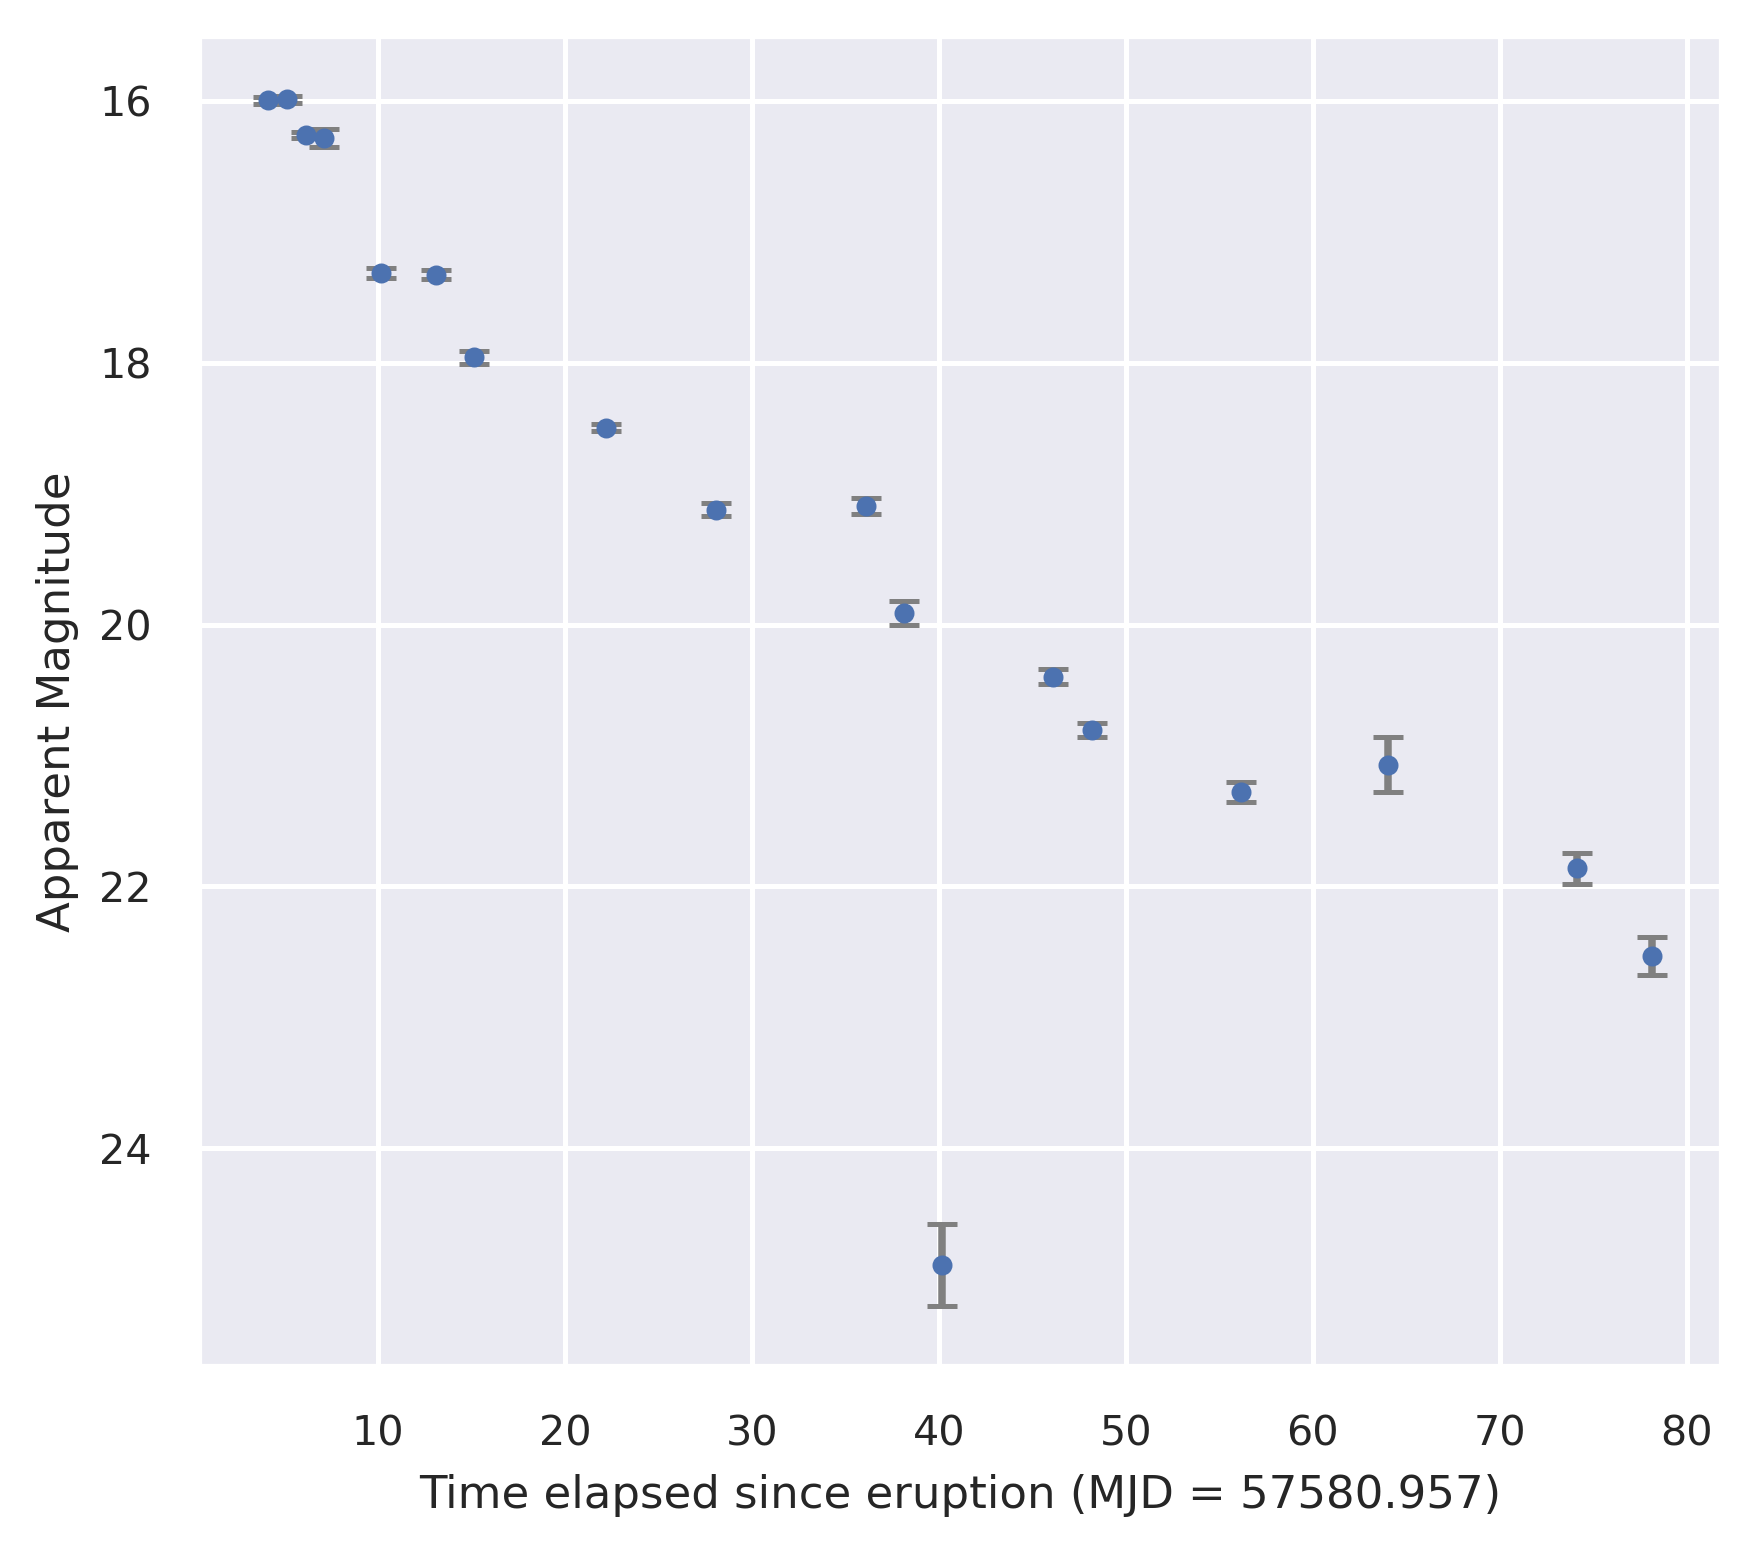
\includegraphics[width=\linewidth]{../codes/plots/photometry_light_curve.png}
			\caption{The calculated \textit{r'}-band light curve for the nova.}
			\label{fig:light_curve}
		\end{subfigure}
		\caption{Plot used for estimation of optimal aperture size for image and the light curve of the nova.}
	\end{figure}

	Using the same procedure, values of optimal apertures for each image can be calculated and are summarized in table \ref{table:aperture_and_span}. These values vary for different images depending upon several factors like atmospheric seeing (or the background noise), object brightness, exposure time, etc.

	To obtain photometric measurements for the nova, we need to compare its brightness to that of standard stars, whose true photometric measurements, under \emph{idealized} conditions are already known and publicly available in catalogs. Accordingly, five secondary standards stars, given their availability in our field of view, are selected to calibrate our photometry of nova. Their IDs in the catalog provided, along with their corresponding approximate positional coordinates on image grid are given in table \ref{table:secondary_standards}. We need to consider only the stars which have been observed to remain static (i.e. not a variable star) over extremely long periods, so that its low photometric uncertainty can be considered reliable for calibration. Even if the atmospheric seeing is unfavourable, photometry can still be performed if we can safely assume that the extent of unfavourability of conditions is similar for both the objects (-- nova being studied and the standard star), which is a reasonable assumption for the nearby secondary standards. Secondly, slightly distant secondary stars in the field of view can be used to estimate variabilities in atmospheric extinction across field of view. For observing faint events, exposure times are often long enough to primary standards. Somewhat dimmer secondary standards are therefore more helpful in these cases.

	A large number of PS1 secondary standard stars are available in field of view. However, not all of them are suitable enough to be used in our case. Parameters like vicinity to the nova and brightness comparable to that of our nova help in selection of most suitable standard stars. Vicinity leads to correlating atmospheric extinction for the two objects. Comparable brightness or \emph{spread} of stars aids the use of same aperture for all standard stars as well as the nova in the image. It must be noted that every secondary star selected should be capable of being resolved properly in the images.

	Equipped with the procedure followed so far, we can obtain photometry of nova as well as the five secondary standards. The obtained apparent magnitudes (\(m_{nova}\) and \(m_{star}\)) are given in table \ref{table:photometry_nova_stars}.

	\begin{table}
		\centering
		\begin{tabular} {l c c c c c c c}
			\toprule
			\textbf{Star} & \textbf{Catalog ID} & \textbf{Position} & \textbf{r} & \textbf{r error} & \textbf{g} & \textbf{g error} & \textbf{r'} \\
			\midrule
			Star 1 & 11 & (1079,741) & 16.1868 & 0.0044 & 16.8984 & 0.0052 & 16.194 \\
			Star 2 & 2 & (985,665) & 16.7696 & 0.0065 & 17.5087 & 0.0059 & 16.777 \\
			Star 3 & 6 & (740,1205) & 16.5210 & 0.0066 & 16.9415 & 0.0034 & 16.525 \\
			Star 4 & 30 & (392,1111) & 18.1143 & 0.0062 & 18.5278 & 0.0049 & 18.118 \\
			Star 5 & 10 & (1275,1305) & 15.7283 & 0.0020 & 16.0337 & 0.0042 & 15.731 \\
			\bottomrule
		\end{tabular}
		\caption{PS1 catalog IDs and approximate positional coordinates of secondary standards used for calibrating photometry of nova.}
		\label{table:secondary_standards}
	\end{table}

	\begin{table}
		\centering
		\begin{tabular} {r r r r r r}
			\toprule
			\textbf{Nova} & \textbf{Star 1} & \textbf{Star 2} & \textbf{Star 3} & \textbf{Star 4} & \textbf{Star 5} \\
			\midrule
			-8.069 \(\pm\) 0.006 & -8.792 \(\pm\) 0.003 & -8.193 \(\pm\) 0.005 & -8.432 \(\pm\) 0.004 & -6.820 \(\pm\) 0.016 & -9.235 \(\pm\) 0.002 \\
			-8.118 \(\pm\) 0.005 & -9.086 \(\pm\) 0.002 & -8.492 \(\pm\) 0.004 & -8.727 \(\pm\) 0.003 & -7.117 \(\pm\) 0.011 & -9.522 \(\pm\) 0.002 \\
			-7.788 \(\pm\) 0.007 & -8.949 \(\pm\) 0.003 & -8.348 \(\pm\) 0.004 & -8.585 \(\pm\) 0.003 & -6.954 \(\pm\) 0.013 & -9.379 \(\pm\) 0.002 \\
			-7.750 \(\pm\) 0.007 & -9.066 \(\pm\) 0.002 & -8.472 \(\pm\) 0.004 & -8.710 \(\pm\) 0.003 & -7.093 \(\pm\) 0.125 & -9.510 \(\pm\) 0.001 \\
			-7.014 \(\pm\) 0.016 & -8.672 \(\pm\) 0.004 & -8.078 \(\pm\) 0.006 & -8.330 \(\pm\) 0.005 & -6.729 \(\pm\) 0.020 & -9.109 \(\pm\) 0.003 \\
			-6.795 \(\pm\) 0.016 & -8.761 \(\pm\) 0.003 & -8.170 \(\pm\) 0.005 & -8.411 \(\pm\) 0.004 & -6.801 \(\pm\) 0.016 & -9.201 \(\pm\) 0.002 \\
			-6.225 \(\pm\) 0.026 & -8.443 \(\pm\) 0.003 & -7.863 \(\pm\) 0.006 & -8.095 \(\pm\) 0.005 & -6.459 \(\pm\) 0.021 & -8.870 \(\pm\) 0.003 \\
			-6.003 \(\pm\) 0.010 & -8.784 \(\pm\) 0.002 & -8.199 \(\pm\) 0.003 & -8.448 \(\pm\) 0.002 & -6.839 \(\pm\) 0.006 & -9.238 \(\pm\) 0.002 \\
			-5.190 \(\pm\) 0.031 & -8.447 \(\pm\) 0.003 & -7.868 \(\pm\) 0.004 & -8.105 \(\pm\) 0.003 & -6.488 \(\pm\) 0.010 & -8.890 \(\pm\) 0.002 \\
			-5.316 \(\pm\) 0.046 & -9.070 \(\pm\) 0.002 & -8.475 \(\pm\) 0.003 & -8.721 \(\pm\) 0.003 & -7.120 \(\pm\) 0.009 & -9.512 \(\pm\) 0.002 \\
			-4.584 \(\pm\) 0.072 & -8.588 \(\pm\) 0.003 & -8.007 \(\pm\) 0.004 & -8.269 \(\pm\) 0.003 & -6.6333 \(\pm\) 0.012 & -9.035 \(\pm\) 0.002 \\
			0.351 \(\pm\) 0.284 & -7.629 \(\pm\) 0.007 & -7.0654 \(\pm\) 0.012 & -7.293 \(\pm\) 0.010 & -5.638 \(\pm\) 0.041 & -8.089 \(\pm\) 0.005 \\
			-4.087 \(\pm\) 0.038 & -8.717 \(\pm\) 0.002 & -8.138 \(\pm\) 0.003 & -8.385 \(\pm\) 0.002 & -6.775 \(\pm\) 0.005 & -9.163 \(\pm\) 0.002 \\
			-3.757 \(\pm\) 0.037 & -8.403 \(\pm\) 0.002 & -7.811 \(\pm\) 0.003 & -8.072 \(\pm\) 0.003 & -6.452 \(\pm\) 0.006 & -8.851 \(\pm\) 0.002 \\
			-3.280 \(\pm\) 0.056 & -8.462 \(\pm\) 0.002 & -7.897 \(\pm\) 0.003 & -8.153 \(\pm\) 0.003 & -6.525 \(\pm\) 0.006 & -8.933 \(\pm\) 0.002 \\
			-3.371 \(\pm\) 0.193 & -8.819 \(\pm\) 0.002 & -8.214 \(\pm\) 0.003 & -8.463 \(\pm\) 0.003 & -6.862 \(\pm\) 0.009 & -9.251 \(\pm\) 0.002 \\
			-2.690 \(\pm\) 0.103 & -8.512 \(\pm\) 0.001 & -7.917 \(\pm\) 0.002 & -8.173 \(\pm\) 0.001 & -6.534 \(\pm\) 0.004 & -8.959 \(\pm\) 0.001 \\
			-1.997 \(\pm\) 0.128 & -8.089 \(\pm\) 0.001 & -7.494 \(\pm\) 0.002 & -7.763 \(\pm\) 0.002 & -6.098 \(\pm\) 0.005 & -8.518 \(\pm\) 0.001 \\
			\bottomrule
		\end{tabular}
		\caption{Values of apparent magnitudes (rounded off to three decimal places) and corresponding error estimates obtained for nova and secondary stars corresponding to the 18 photometric images.}
		\label{table:photometry_nova_stars}
	\end{table}

	\begin{table}
		\centering
		\begin{tabular} {l r r r r r}
			\toprule
			\textbf{Airmass} & \textbf{Star 1} & \textbf{Star 2} & \textbf{Star 3} & \textbf{Star 4} & \textbf{Star 5} \\
			\midrule
			1.7258 & 24.985 \(\pm\) 0.007 & 24.970 \(\pm\) 0.009 & 24.956 \(\pm\) 0.008 & 24.937 \(\pm\) 0.020 & 15.992 \(\pm\)  0.026 \\
			1.6665 & 25.280 \(\pm\) 0.006 & 25.268 \(\pm\) 0.007 & 25.251 \(\pm\) 0.006 & 25.235 \(\pm\) 0.015 & 15.985 \(\pm\)  0.023 \\
			1.7491 & 25.143 \(\pm\) 0.006 & 25.124 \(\pm\) 0.008 & 25.109 \(\pm\) 0.007 & 25.072 \(\pm\) 0.017 & 16.257 \(\pm\)  0.026 \\
			1.7721 & 25.260 \(\pm\) 0.006 & 25.249 \(\pm\) 0.007 & 25.234 \(\pm\) 0.007 & 25.210 \(\pm\) 0.129 & 16.279 \(\pm\)  0.069 \\
			1.3530 & 24.866 \(\pm\) 0.007 & 24.855 \(\pm\) 0.010 & 24.854 \(\pm\) 0.009 & 24.846 \(\pm\) 0.024 & 17.312 \(\pm\)  0.038 \\
			1.6443 & 24.954 \(\pm\) 0.007 & 24.946 \(\pm\) 0.008 & 24.936 \(\pm\) 0.007 & 24.918 \(\pm\) 0.019 & 17.323 \(\pm\)  0.035 \\
			1.5562 & 24.637 \(\pm\) 0.007 & 24.639 \(\pm\) 0.010 & 24.619 \(\pm\) 0.009 & 24.577 \(\pm\) 0.025 & 17.956 \(\pm\)  0.048 \\
			1.1115 & 24.978 \(\pm\) 0.005 & 24.976 \(\pm\) 0.006 & 24.972 \(\pm\) 0.006 & 24.957 \(\pm\) 0.009 & 18.493 \(\pm\)  0.026 \\
			1.3717 & 24.641 \(\pm\) 0.006 & 24.645 \(\pm\) 0.007 & 24.630 \(\pm\) 0.007 & 24.605 \(\pm\) 0.014 & 19.122 \(\pm\)  0.049 \\
			1.2355 & 25.264 \(\pm\) 0.006 & 25.252 \(\pm\) 0.007 & 25.245 \(\pm\) 0.006 & 25.242 \(\pm\) 0.013 & 19.092 \(\pm\)  0.063 \\
			1.1156 & 24.781 \(\pm\) 0.006 & 24.783 \(\pm\) 0.008 & 24.793 \(\pm\) 0.007 & 24.750 \(\pm\) 0.015 & 19.910 \(\pm\)  0.090 \\
			1.0482 & 23.823 \(\pm\) 0.011 & 23.842 \(\pm\) 0.015 & 23.818 \(\pm\) 0.013 & 23.756 \(\pm\) 0.044 & 24.893 \(\pm\)  0.313 \\
			1.1306 & 24.911 \(\pm\) 0.005 & 24.915 \(\pm\) 0.006 & 24.910 \(\pm\) 0.006 & 24.893 \(\pm\) 0.009 & 20.396 \(\pm\)  0.054 \\
			1.0244 & 24.597 \(\pm\) 0.006 & 24.588 \(\pm\) 0.007 & 24.597 \(\pm\) 0.006 & 24.569 \(\pm\) 0.010 & 20.802 \(\pm\)  0.054 \\
			1.0250 & 24.655 \(\pm\) 0.006 & 24.673 \(\pm\) 0.006 & 24.677 \(\pm\) 0.006 & 24.643 \(\pm\) 0.009 & 21.278 \(\pm\)  0.073 \\
			1.1904 & 25.012 \(\pm\) 0.006 & 24.991 \(\pm\) 0.007 & 24.988 \(\pm\) 0.006 & 24.979 \(\pm\) 0.012 & 21.070 \(\pm\)  0.210 \\
			1.0329 & 24.706 \(\pm\) 0.005 & 24.694 \(\pm\) 0.005 & 24.697 \(\pm\) 0.005 & 24.651 \(\pm\) 0.008 & 21.862 \(\pm\)  0.119 \\
			1.0706 & 24.283 \(\pm\) 0.005 & 24.270 \(\pm\) 0.006 & 24.287 \(\pm\) 0.006 & 24.216 \(\pm\) 0.009 & 22.529 \(\pm\)  0.145 \\
			\bottomrule
		\end{tabular}
		\caption{Values of airmass and zero-point, Z (given by equation \ref{eq:Z}), with corresponding error estimates for each of the 18 image files in sequence. Values of Z are truncated to three decimal places for representation.}
		\label{table:Z_airmass}
	\end{table}



	In order to use the photometric measurements provided in the PS1 catalog, we need to translate values presented in PS1 system to SDSS system as mentioned in the handout. This conversion is performed in table \ref{table:secondary_standards} using the relation \citep{2012ApJ...750...99T}:
	 \begin{equation}
	 	r' = r-0.001+0.11(g-r) \pm 0.004
	 \end{equation} 

	Now, we use the following equation to obtain values of zero-point for each observation, given by \(Z\) in the following equation. The values computed are given in table \ref{table:Z_airmass}.
	\begin{equation}
	 	Z = r' - m_{star}
	 	\label{eq:Z}
	\end{equation} 
	Now, for each star, we use the values of Z from table \ref{table:Z_airmass} and find the best fit line for them. Then, we calculate the slope of the best-fit line and evaluate the value of Z at the value of airmass equal to 1. These values for each secondary star are summarised in table \ref{table:slope_Z1}.

	\begin{table}
		\centering
		\begin{tabular} {l r r}
			\toprule
			\textbf{star} & \textbf{Z at airmass 1} & \textbf{slope} \\
			\midrule
			1 & 24.58518 & 0.72978 \\
			2 & 24.58542 & 0.71267 \\
			3 & 24.58767 & 0.68760 \\
			4 & 24.55271 & 0.70689 \\
			5 & 24.57150 & 0.71021\\
			\bottomrule
		\end{tabular}
		\caption{Value of Z at airmass 1 and the slope of best fit line to the values of Z for each secondary standard star.}
		\label{table:slope_Z1}
	\end{table}

	The magnitude of nova obtained using each secondary standard star (\(m^{star}_{nova}\)) can now be obtained using the equation,
	\begin{equation}
		m^{star}_{nova} = Z_{star} + m_{nova} - C_{airmass},
	\end{equation}
	where \(C_{airmass}\) is the airmass correction given by,
	\begin{equation}
		C_{airmass} = (\textrm{airmass} -1) \times \textrm{slope}.
	\end{equation}

	Using this methodology, we obtain the magnitude of nova in each image by using a set of five secondary stars. These values obtained using each standard star, are given in table \ref{table:photometry_nova}. Given that the values obtained at each epoch seem to be roughly similar within the limits of errors and uncertainties, we can be sure that the performed photometry is consistent, and indeed a suitable choice of secondary stars was made. We now use the mean of these values obtained at each epoch to plot the light-curve given in figure \ref{fig:light_curve}.

	On the basis of classification of nova light curves by \citet{2010AJ....140...34S} the shape appears to be that of a smooth light curve with no oscillations, flat top, cusp or any signs of dust dip within the \(\sim 80\) days period of observation. Light curve can be represented by a power-law. The extreme variation in photometry around day 11 is probably due to poor photometric conditions and should not be confused for a dust dip because of two reasons -- the variation in magnitude is small compared to typical examples of dust-dip light curves and such a dip is not retained on any of the further observations and cannot be such short lived.

	\begin{table}
		\centering
		\begin{tabular} {r r r r r r}
			\toprule
			\textbf{From Star 1} & \textbf{From Star 2} & \textbf{From Star 3} & \textbf{From Star 4} & \textbf{From Star 5} & \textbf{Mean}\\
			\midrule
			15.986 \(\pm\) 0.022 & 15.998 \(\pm\) 0.026 & 16.019 \(\pm\) 0.023 & 15.970 \(\pm\) 0.037 & 15.986 \(\pm\) 0.017 & 15.992 \(\pm\) 0.127 \\
			15.980 \(\pm\) 0.020 & 15.992 \(\pm\) 0.024 & 16.011 \(\pm\) 0.021 & 15.963 \(\pm\) 0.030 & 15.980 \(\pm\) 0.016 & 15.985 \(\pm\) 0.114 \\
			16.250 \(\pm\) 0.022 & 16.263 \(\pm\) 0.027 & 16.284 \(\pm\) 0.023 & 16.235 \(\pm\) 0.035 & 16.251 \(\pm\) 0.018 & 16.257 \(\pm\) 0.127 \\
			16.272 \(\pm\) 0.023 & 16.285 \(\pm\) 0.027 & 16.307 \(\pm\) 0.024 & 16.257 \(\pm\) 0.147 & 16.273 \(\pm\) 0.019 & 16.279 \(\pm\) 0.241 \\
			17.313 \(\pm\) 0.033 & 17.320 \(\pm\) 0.038 & 17.331 \(\pm\) 0.034 & 17.289 \(\pm\) 0.051 & 17.306 \(\pm\) 0.028 & 17.312 \(\pm\) 0.186 \\
			17.319 \(\pm\) 0.032 & 17.330 \(\pm\) 0.036 & 17.348 \(\pm\) 0.033 & 17.301 \(\pm\) 0.046 & 17.318 \(\pm\) 0.027 & 17.323 \(\pm\) 0.176 \\
			17.954 \(\pm\) 0.043 & 17.963 \(\pm\) 0.048 & 17.980 \(\pm\) 0.045 & 17.934 \(\pm\) 0.062 & 17.951 \(\pm\) 0.039 & 17.956 \(\pm\) 0.239 \\
			18.500 \(\pm\) 0.025 & 18.502 \(\pm\) 0.028 & 18.507 \(\pm\) 0.026 & 18.470 \(\pm\) 0.030 & 18.488 \(\pm\) 0.021 & 18.493 \(\pm\) 0.133 \\
			19.123 \(\pm\) 0.047 & 19.130 \(\pm\) 0.051 & 19.141 \(\pm\) 0.048 & 19.099 \(\pm\) 0.056 & 19.117 \(\pm\) 0.043 & 19.122 \(\pm\) 0.246 \\
			19.096 \(\pm\) 0.061 & 19.101 \(\pm\) 0.065 & 19.109 \(\pm\) 0.062 & 19.069 \(\pm\) 0.070 & 19.087 \(\pm\) 0.057 & 19.092 \(\pm\) 0.317 \\
			19.916 \(\pm\) 0.087 & 19.918 \(\pm\) 0.092 & 19.924 \(\pm\) 0.088 & 19.886 \(\pm\) 0.098 & 19.905 \(\pm\) 0.083 & 19.910 \(\pm\) 0.451 \\
			24.901 \(\pm\) 0.305 & 24.902 \(\pm\) 0.312 & 24.905 \(\pm\) 0.308 & 24.869 \(\pm\) 0.340 & 24.888 \(\pm\) 0.299 & 24.893 \(\pm\) 1.565 \\
			20.402 \(\pm\) 0.053 & 20.405 \(\pm\) 0.057 & 20.410 \(\pm\) 0.054 & 20.373 \(\pm\) 0.058 & 20.391 \(\pm\) 0.050 & 20.396 \(\pm\) 0.274 \\
			20.810 \(\pm\) 0.053 & 20.811 \(\pm\) 0.056 & 20.814 \(\pm\) 0.054 & 20.778 \(\pm\) 0.058 & 20.797 \(\pm\) 0.049 & 20.802 \(\pm\) 0.272 \\
			21.286 \(\pm\) 0.072 & 21.287 \(\pm\) 0.075 & 21.290 \(\pm\) 0.072 & 21.255 \(\pm\) 0.077 & 21.273 \(\pm\) 0.068 & 21.278 \(\pm\) 0.365 \\
			21.074 \(\pm\) 0.208 & 21.078 \(\pm\) 0.212 & 21.085 \(\pm\) 0.209 & 21.046 \(\pm\) 0.216 & 21.065 \(\pm\) 0.204 & 21.070 \(\pm\) 1.051 \\
			21.870 \(\pm\) 0.118 & 21.871 \(\pm\) 0.121 & 21.874 \(\pm\) 0.118 & 21.838 \(\pm\) 0.122 & 21.857 \(\pm\) 0.114 & 21.862 \(\pm\) 0.595 \\
			22.536 \(\pm\) 0.144 & 22.537 \(\pm\) 0.147 & 22.541 \(\pm\) 0.144 & 22.505 \(\pm\) 0.149 & 22.524 \(\pm\) 0.140 & 22.529 \(\pm\) 0.726 \\
			\bottomrule
		\end{tabular}
		\caption{Apparent magnitudes of nova at sequential epochs along with the estimated uncertainties calculated using standard secondary stars.}
		\label{table:photometry_nova}
	\end{table}


	Assuming that the peak occurred on approximately the same time as our first observation (which is roughly the brightest observation), we get the approximate value of peak apparent magnitude, \(m_0 \approx 16\) at time, \(t_0 \approx 4.122\) days post-eruption.
	Therefore, \(t_2 = 10.986\) days \(t_3 = 34.30\) days and \(m_{15} = 18.25\).

	Maximum magnitude rate of decline (MMRD) relationships for \textit{V}-band magnitudes involving \(t_2\) and \(t_3\) are given as \citep{2000AJ....120.2007D}:
	\begin{equation}
		M_V = (-11.32 \pm 0.44) + (2.55 \pm 0.32) \log t_2 ,
		\label{eq:t2_mmrd}
	\end{equation}
	\begin{equation}
		M_V = (-11.99 \pm 0.56) + (2.54 \pm 0.35) \log t_3.
		\label{eq:t3_mmrd}
	\end{equation}

	If we assume that these relations hold approximately true to \textit{r'}-band absolute magnitudes also \citep{2006MNRAS.369..257D}, we can estimate distance to the nova using the distance modulus equation given by,
	\begin{equation}
		m_{r'} - M_{r'} = 5 \log d - 5 + A_{r'},
		\label{eq:distance_modulus}
	\end{equation}
	where, \(A_{r'}\) is the not yet known extinction correction term and thereby assumed to b equal to 0.
	Using equation \ref{eq:t2_mmrd}, we obtain,
	\[M_{r'}^{t_2} \approx -8.663 \pm 0.773 \] 
	Using equation \ref{eq:t3_mmrd}, we obtain,
	\[M_{r'}^{t_3} \approx -8.090 \pm 1.098\]
	Using the value of \(M_{r'}^{t_2}\), \(d_{t_2} = 857.43^{+366.62}_{-256.81} \) kpc. \\
	Using the value of \(M_{r'}^{t_3}\), \(d_{t_3} = 657.66^{+432.78}_{-260.83}\) kpc. \\

	The \(t_{15}\) relation by \citet{2003ApJ...599.1302F} states that, the absolute magnitude of a nova, 15 days post maximum is given by,
	\begin{equation}
		M_{V}^{t_{15}} = -6.36 \pm 0.29
		\label{eq:t15_mmrd}
	\end{equation}
	Once again, if we assume that this relation holds true for \textit{r'}-band magnitudes also, then using the value of \(M_{r'}^{t_{15}}\), we estimate the distance to the nova as, \(d_{t_{15}} = 835.60^{+119.39}_{-104.46}\) kpc. \\


%	======================================= Spectroscopy ====================================
	
	\subsection{Spectroscopy} \label{sec:spectroscopy}

	To study the spectral evolution of the nova, the \texttt{splat} software is used, which is also a part of the Starlink suite of software applications. A spectrum is a plot of power per unit area, per unit wavelength (flux density) as a function of wavelength, which essentially tells us the distribution of energy as a function of wavelength. This is indicated by the units assigned to x and y-axes, \textit{i.e.} erg s\(^{-1}\) cm\(^{-2}\) \r{A}\(^{-1}\) and \r{A}, respectively, where an \emph{erg} is a unit of energy, numerically equal to \(10^{-7}\)Joules.

	When a spectrum is  viewed in the \texttt{splat} software, one can see and identify five major components in the spectral plot.
	\begin{itemize}
		\item Continuum emission from thermal radiations emitted over a large wavelength range by the inner dense material. 
		\item Emission lines from radiation emitted by surrounding ejecta which absorbs wavelengths from continuum and emits at specific wavelengths. 
		\item Absorption lines from radiation absorbed by the column of interstellar medium (ISM) in our line of sight of nova. 
		\item Cosmic rays of galactic, extra-galactic and solar origins. 
		\item Statistical noise inherent to measurements from instruments. Also called shot noise, it doesn't have any fixed pattern.
	\end{itemize}

	The most prominent of these features, the emission lines, are essentially the \emph{recombination lines} formed when an ion captures a free electron. The electron is captured at higher energy levels of the ion and then \emph{cascades} down to lower energy levels, thereby emitting at multiple wavelengths. The least prominent of all features, which require zooming in at specific wavelengths, are the ISM absorption lines that are formed due to absorption at specific wavelength by cold gas of extremely low density. Dust containing metals also absorbs certain wavelengths depending upon the metals contained in the grains. Statistical noise and Cosmic ray hits, on the other hand, are random features and differ in intensities and locations across different exposures randomly. 

	One thing to note is that at each epoch, three short exposures are obtained by the SPRAT module on Liverpool Telescope, instead of one (3x) long exposure. Although this has one disadvantage of slight increase in readout noise, there are several advantages which far outweigh the disadvantages. Multiple exposure prevent the saturation of CCD units by brightest features and can also be used to remove random defects. More importantly, the cosmic ray hits and transient bright objects in the sky (asteroids, satellites, etc.) can be easily located and handled accordingly. 

	Cosmic ray hits, which occur at random energies (wavelengths), can be removed from the spectra if multiple exposures are available by taking the median value at each point. This approach of median stacking, however, does not work for statistical noise, which is seen at every wavelength.

	We can begin our spectral analysis by taking median value of three exposures at each epoch. The removal of cosmic ray hits can be observed once this is done following the procedure mentioned in the handout. We can then compare the time-evolution of the five components mentioned above, by observing trends across the 10 spectra now available to us. 

	\begin{itemize}
		\item Continuum emission reduces in strength over time. The reduction is more prominent in the earlier spectra.
		\item Emission lines also reduce in strength over time more prominently in the earlier spectra. Some weaker emissions fade completely over time.
		\item ISM absorption is comparatively stronger when continuum emission is stronger. With passing time absorption fades.
		\item Cosmic ray hits remain constant, but their occurrence has been removed from spectra upon taking median for each epoch, given their insignificance in our study.
		\item Statistical noise appears to increase slightly as we go to later spectra. However, that appears due to reduction in value of SNR over time.
	\end{itemize}

	To summarize our work so far, we have used median stacking process for all 10 epochs using multiple exposures. This has removed cosmic ray signatures almost entirely, while statistical noise has not seen any major change. All other components have been preserved although extremely small signals may now seem lost in the statistical noise. We know now that the strength of continuum fades over time. Given that its presence is not much significant any further in our study, which comprises primarily of emission lines and ISM absorption lines, we can remove the continuum by fitting an approximate function that imitates its profile, and then subtract it from the spectrum. Such a spectrum is called a \emph{continuum subtracted spectrum}. In our case, a polynomial of degree 3 gave the best improvement in reduction of root-mean-square error and was thus used to remove the continuum from spectra at each epoch. To ascertain whether the continuum has been appropriately subtracted, we repeat the procedure of continuum removal once again. This time, we get a continuum fitting curve which is a horizontal line corresponding to zero flux density, indicating that continuum has been successfully removed. Using a higher order polynomial for this purpose also gave insignificant fitting values.

	A number of emission lines can new be easily recognized in each spectrum, some of which correspond to emissions from H \textsc{\romannumeral 1} (H \textsc{\(\delta\)}, H \textsc{\(\gamma\)}, H \textsc{\(\beta\)}, H \textsc{\(\alpha\)}), Fe \textsc{\romannumeral 2} (42,48,49), O \textsc{\romannumeral 1} (1,21,55) and possibly Si \textsc{\romannumeral 2} (4). Using classification provided by \citet{2012AJ....144...98W}, we can conclude that nova is of Fe \textsc{\romannumeral 2} spectroscopic class.

	It is known that effects of interstellar extinction are prevalent over a continuous wavelength range. However, we can identify two interstellar absorption lines, which are collectively called the Na \textsc{\romannumeral 1} doublet corresponding to wavelengths 5889.95\r{A} (D2) and 5895.92\r{A} (D1). By fitting Lorentzian line profiles to these two absorption lines, we can estimate the flux absorbed. The interstellar reddening E(B--V) can be calculated using the equations \citep{na_abs_line},
	\begin{equation}
		\log \left[ E(B-V) \right] = 2.16 \times \textrm{EW}(\textrm{D2}) -1.91 \pm 0.15 ,
	\end{equation}
	\begin{equation}
		\log \left[ E(B-V) \right] = 2.47 \times \textrm{EW}(\textrm{D1}) -1.76 \pm 0.17 ,
	\end{equation}
	where, EW stands for \emph{equivalent width} of corresponding lines, given by,
	\begin{equation}
		\textrm{EW} \approx - \frac{F_{line}}{f_{cont}},
	\end{equation}
	where, \(F_{line}\) is the (negative) flux of absorption line and \(f_{cont}\) is the continuum flux at that wavelength. Using this procedure, the calculated values for the two absorption lines are summarized in table \ref{table:eb-v}. The average value of reddening term computed from the two lines is given by \(\textrm{E(B--V)} = 0.1785 \pm 0.093\).

	\begin{table}
		\centering
		\begin{tabular} {l c c c c}
			\toprule
			\textbf{wavelength} & \textbf{continuum flux} & \textbf{line flux} & \textbf{EW} & \textbf{E(B--V)} \\
			\midrule
			\(5890.009 \pm 0.061\) & \((2.400 \pm 0.1507) \times 10^{-16}\) & \((-1.345 \pm 1.143) \times 10^{-16}\) & 0.560 & \(0.199 \pm 0.069\) \\
			\(5895.935 \pm 0.175\) & \((2.402 \pm 0.1507) \times 10^{-16}\) & \((-0.931 \pm 1.263) \times 10^{-16}\) & 0.388 & \(0.158 \pm 0.062\) \\
			\bottomrule
		\end{tabular}
		\caption{The values of central wavelength, continuum flux, absorption line flux, equivalent widths and interstellar reddening for the two sodium interstellar absorption lines.}
		\label{table:eb-v}
	\end{table}

	While fitting the lines, three different types of line profiles are encountered -- Gaussian, Lorentzian and Voigt. In this study, Lorentzian profile gave the best fit in all cases, with least root-mean-square errors. Voigt profile is essentially a convolution of the other two types of profiles. 

	\begin{table} [b]
		\centering
		\begin{tabular} {r r r r r}
			\toprule
			O \textsc{\romannumeral 1} (1) & \(H \alpha\) & \(H \beta\) & \(H \gamma\) & \(H \delta\) \\
			\midrule
			\((1.96 \pm 0.01) 10^{-13}\) & \((4.95 \pm 0.02) 10^{-13}\) & \((7.58 \pm 0.07)10^{-14}\) & \((3.18 \pm 0.04)10^{-14}\) & \((2.08 \pm 0.03)10^{-14}\) \\
			\((2.98 \pm 0.03) 10^{-14}\) & \((2.75 \pm 0.01) 10^{-13}\) & \((4.08 \pm 0.06)10^{-14}\) & \((1.88 \pm 0.04)10^{-14}\) & \((1.50 \pm 0.04)10^{-14}\) \\
			\((1.55 \pm 0.01) 10^{-14}\) & \((1.70 \pm 0.00) 10^{-13}\) & \((2.49 \pm 0.04)10^{-14}\) & \((1.09 \pm 0.02)10^{-14}\) & \((8.93 \pm 0.29)10^{-15}\) \\
			\((1.12 \pm 0.01) 10^{-14}\) & \((1.27 \pm 0.00) 10^{-13}\) & \((1.85 \pm 0.03)10^{-14}\) & \((8.25 \pm 0.20)10^{-15}\) & \((6.12 \pm 0.20)10^{-15}\) \\
			\((7.30 \pm 0.35) 10^{-15}\) & \((8.41 \pm 0.06) 10^{-14}\) & \((1.19 \pm 0.03)10^{-14}\) & \((5.50 \pm 0.38)10^{-15}\) & \((2.74 \pm 0.40)10^{-15}\) \\
			\((6.70 \pm 0.41) 10^{-15}\) & \((7.87 \pm 0.05) 10^{-14}\) & \((1.08 \pm 0.02)10^{-14}\) & \((5.51 \pm 0.42)10^{-15}\) & \((2.39 \pm 0.81)10^{-15}\) \\
			\((5.83 \pm 0.53) 10^{-15}\) & \((7.23 \pm 0.05) 10^{-14}\) & \((1.00 \pm 0.02)10^{-14}\) & \((3.80 \pm 0.46)10^{-15}\) & \((2.25 \pm 4.81)10^{-15}\) \\
			\((5.88 \pm 1.15) 10^{-15}\) & \((7.25 \pm 0.06) 10^{-14}\) & \((1.01 \pm 0.03)10^{-14}\) & \((4.47 \pm 0.29)10^{-15}\) & \((5.71 \pm 6.09)10^{-15}\) \\
			\((6.59 \pm 1.15) 10^{-15}\) & \((7.07 \pm 0.06) 10^{-14}\) & \((9.50 \pm 0.31)10^{-15}\) & \((5.09 \pm 0.63)10^{-15}\) & \((2.57 \pm 1.08)10^{-15}\) \\
			\((5.21 \pm 1.52) 10^{-15}\) & \((6.77 \pm 0.06) 10^{-14}\) & \((9.14 \pm 0.27)10^{-15}\) & \((4.74 \pm 0.38)10^{-15}\) & \((4.12 \pm 69.0) 10^{-15}\) \\
			\bottomrule
		\end{tabular}
		\caption{Fluxes and associated uncertainties obtained for different emission lines (in units of erg s\(^{-1}\) cm\(^{-2}\) \r{A}\(^{-1}\)) across spectra at all epochs, mentioned sequentially. Values are truncated at two decimal places for representational purpose.}
		\label{table:line_fluxes}
	\end{table}

	\begin{table} [h]
	\centering
		\begin{tabular} {r r r r r}
		\toprule
		O \textsc{\romannumeral 1} (1) & \(H \alpha\) & \(H \beta\) & \(H \gamma\) & \(H \delta\) \\
		\midrule
		\(78.714 \pm 0.634\) & \(51.444 \pm 0.219\) & \(47.185 \pm 0.393\) & \(51.671 \pm 0.620\) & \(51.791 \pm 0.723\) \\
		\(54.016 \pm 0.461\) & \(34.377 \pm 0.129\) & \(32.503 \pm 0.395\) & \(40.518 \pm 0.826\) & \(46.489 \pm 1.218\) \\
		\(40.734 \pm 0.431\) & \(25.816 \pm 0.107\) & \(24.359 \pm 0.347\) & \(27.682 \pm 0.525\) & \(33.247 \pm 0.947\) \\
		\(34.328 \pm 0.425\) & \(21.706 \pm 0.097\) & \(20.642 \pm 0.335\) & \(24.232 \pm 0.518\) & \(25.271 \pm 0.750\) \\
		\(27.558 \pm 1.143\) & \(18.785 \pm 0.120\) & \(17.328 \pm 0.367\) & \(21.666 \pm 1.342\) & \(12.441 \pm 1.722\) \\
		\(28.294 \pm 1.528\) & \(18.681 \pm 0.110\) & \(16.260 \pm 0.368\) & \(22.766 \pm 1.578\) & \(12.364 \pm 4.088\) \\
		\(27.210 \pm 2.297\) & \(18.759 \pm 0.114\) & \(16.619 \pm 0.381\) & \(15.875 \pm 1.816\) & \(12.843 \pm 27.378\) \\
		\(27.340 \pm 5.240\) & \(18.760 \pm 0.129\) & \(16.319 \pm 0.445\) & \(19.282 \pm 1.116\) & \(34.943 \pm 37.214\) \\
		\(33.103 \pm 5.612\) & \(18.822 \pm 0.133\) & \(16.453 \pm 0.458\) & \(23.854 \pm 2.776\) & \(15.605 \pm 6.468\) \\
		\(25.836 \pm 7.491\) & \(18.884 \pm 0.138\) & \(16.123 \pm 0.404\) & \(23.214 \pm 1.677\) & \(8.028 \pm 33.176\) \\
		\bottomrule
		\end{tabular}
		\caption{FWHM and associated uncertainties obtained for different emission lines (in units of \r{A}) across spectra at all epochs, mentioned sequentially.}
		\label{table:line_fwhm}
	\end{table}

	\begin{figure} [h!]
		\centering
		\begin{subfigure} {.49\textwidth}
			\centering
			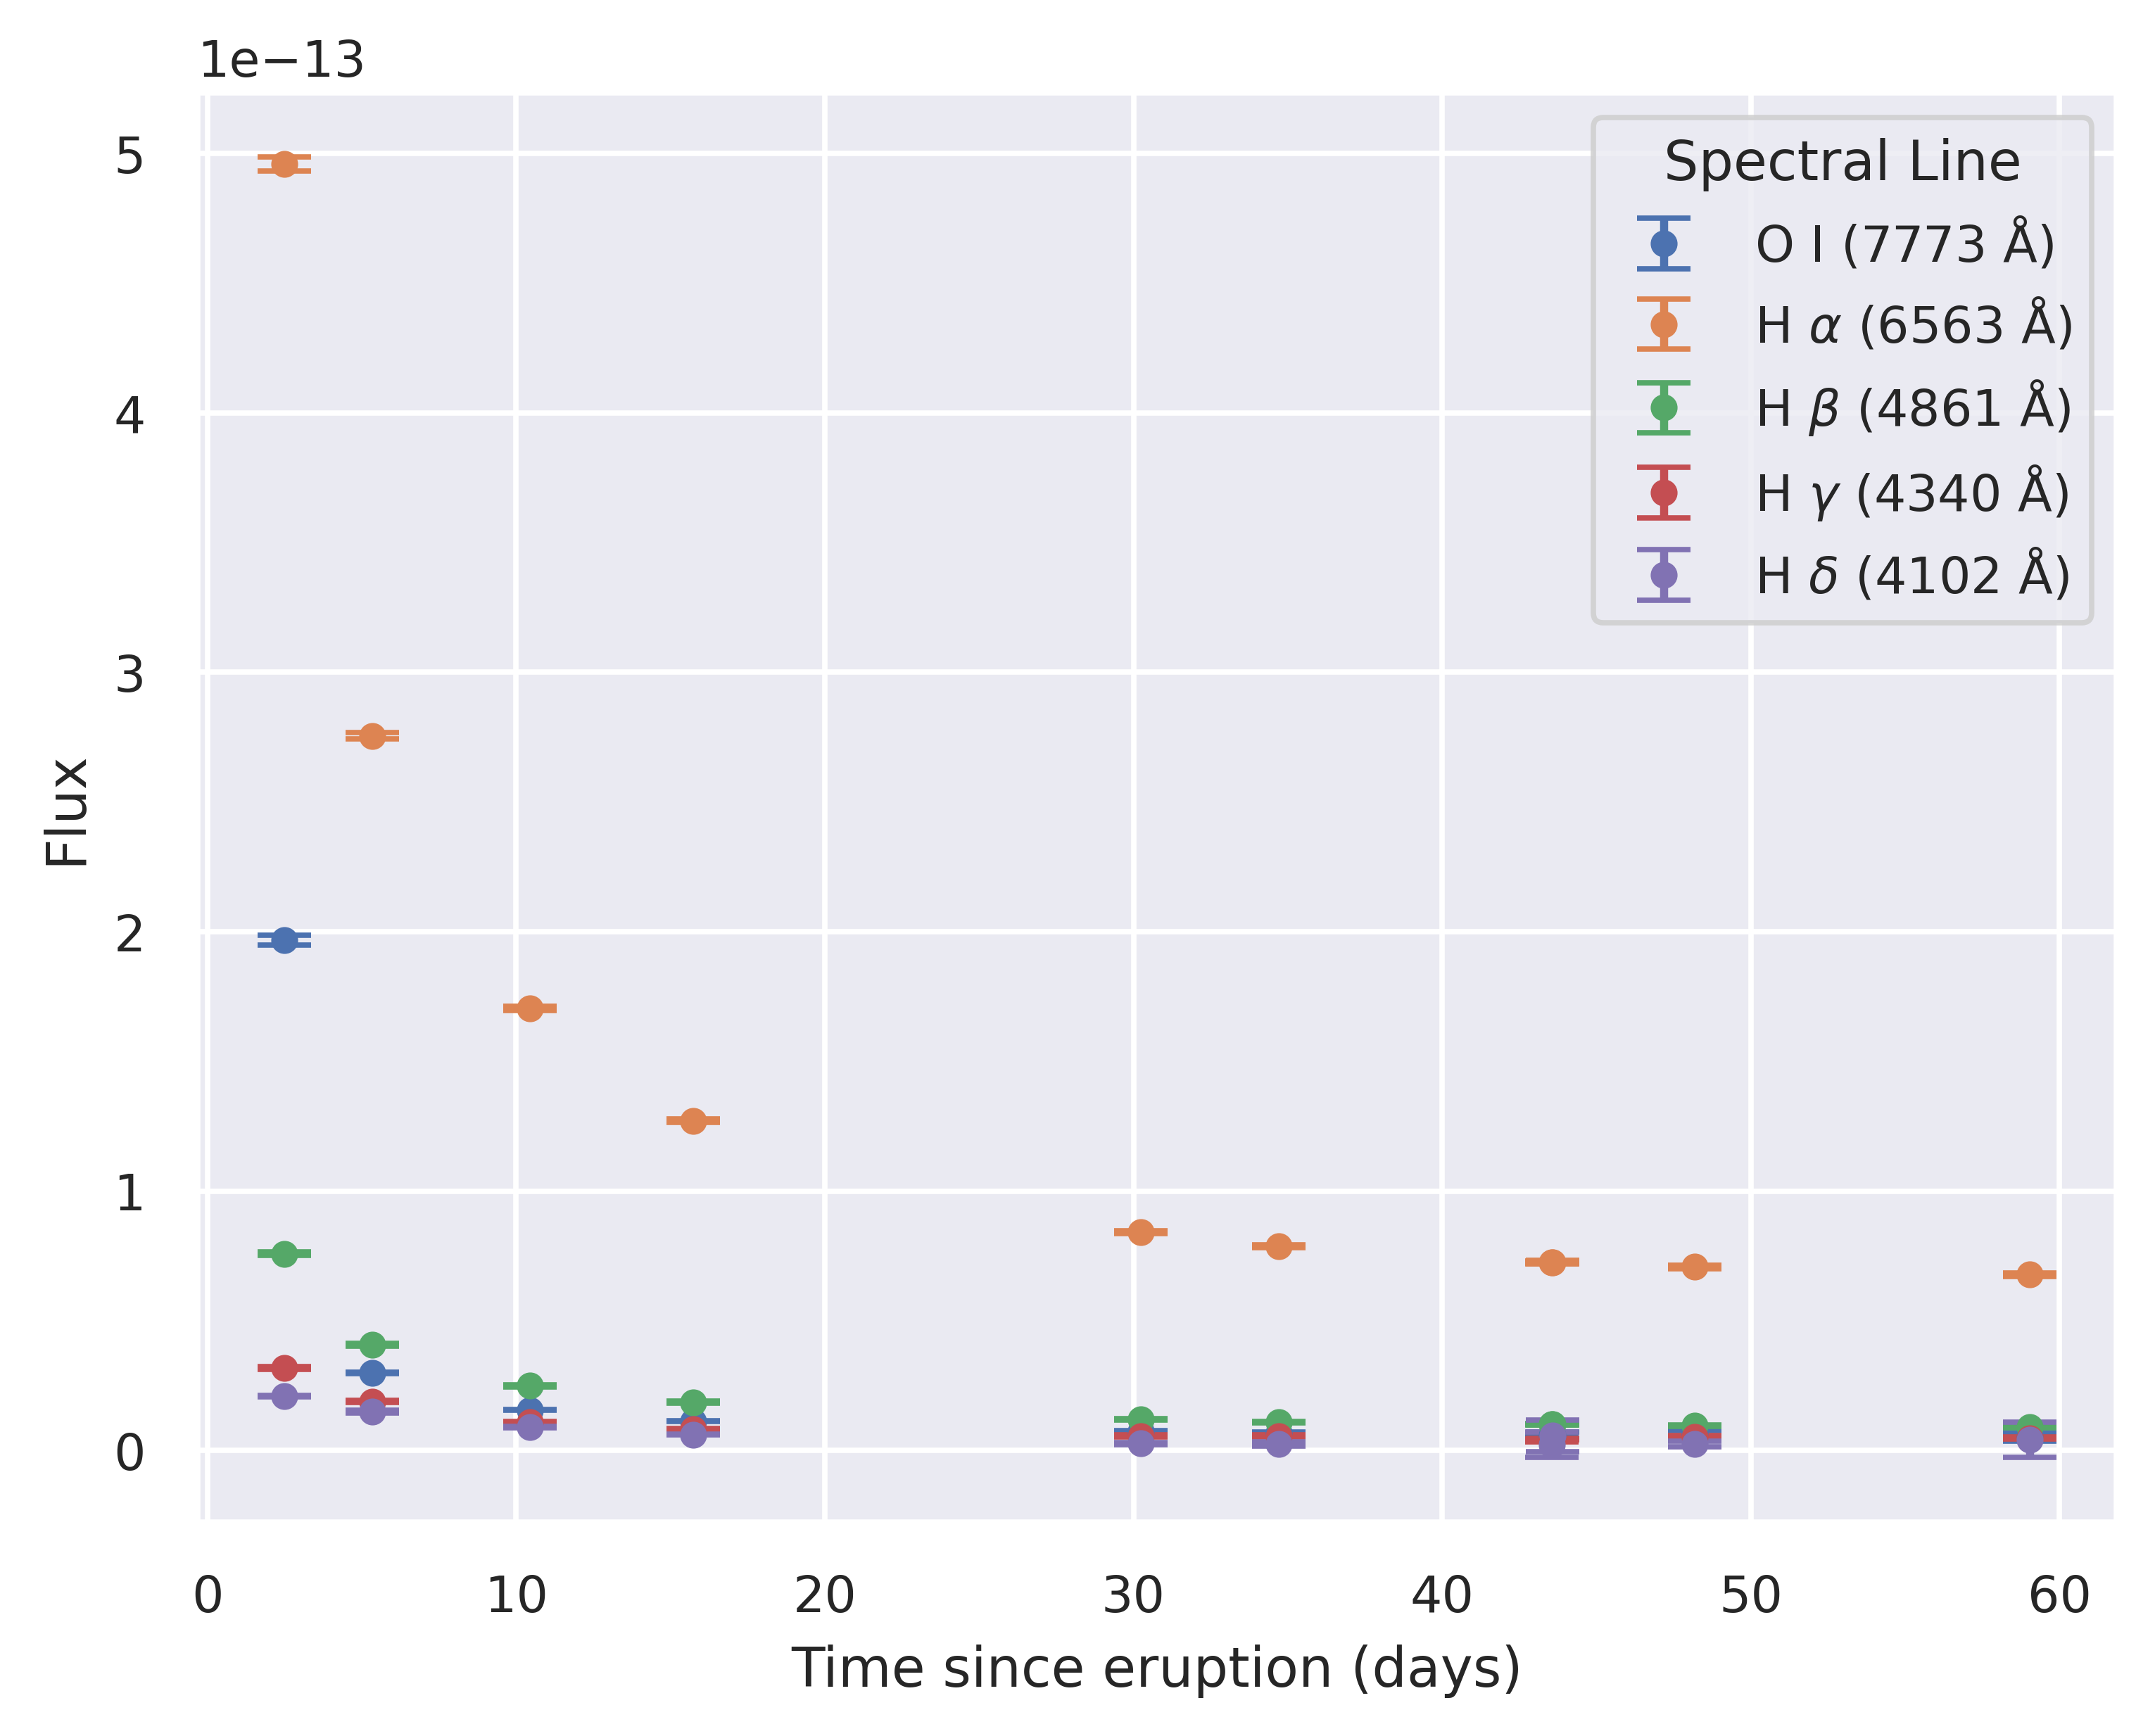
\includegraphics[width=\linewidth]{../codes/plots/line_fluxes_evolution.png}
			\caption{Time evolution of flux (in erg s\(^{-1}\) cm\(^{-2}\) \r{A}\(^{-1}\)) of spectral lines.}
			\label{fig:line_flux_evolution}
		\end{subfigure} %
		\hfill
		\begin{subfigure} {.49\textwidth}
			\centering
			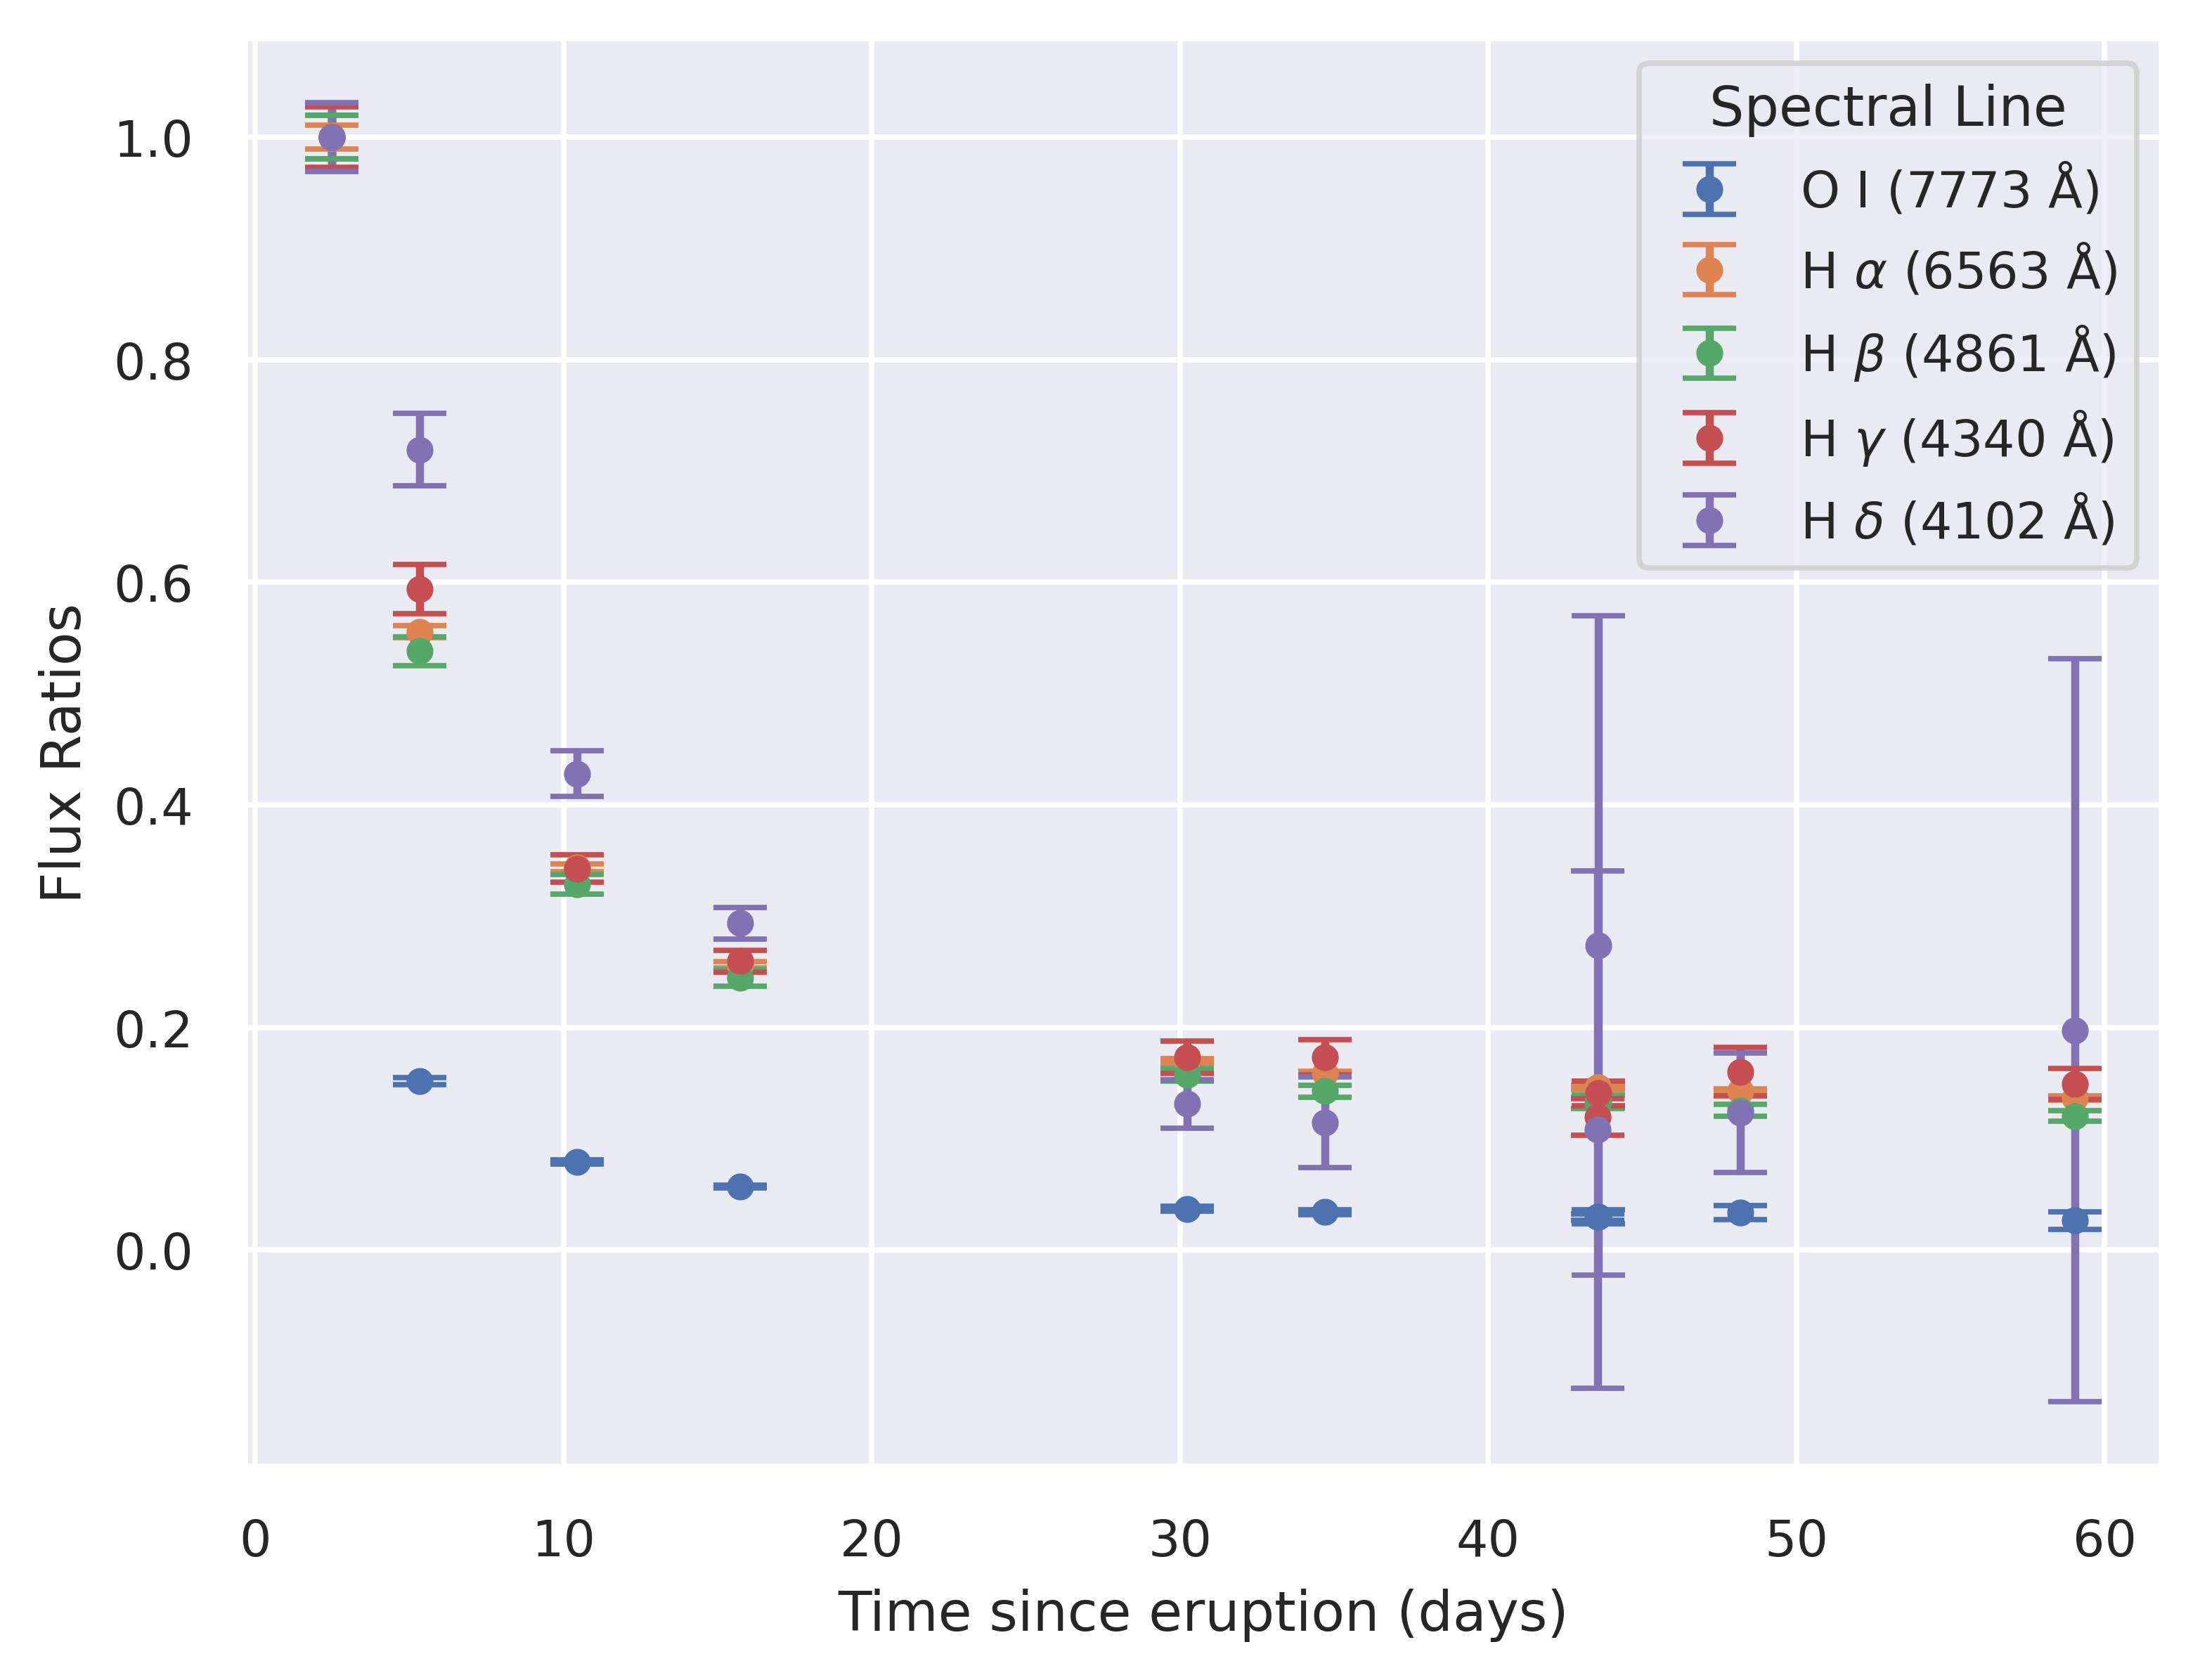
\includegraphics[width=\linewidth]{../codes/plots/line_flux_ratios_evolution.png}
			\caption{Time evolution of flux ratios of spectral lines.}
			\label{fig:flux_ratio_evolution}
		\end{subfigure}
		\begin{subfigure} {.49\textwidth}
			\centering
			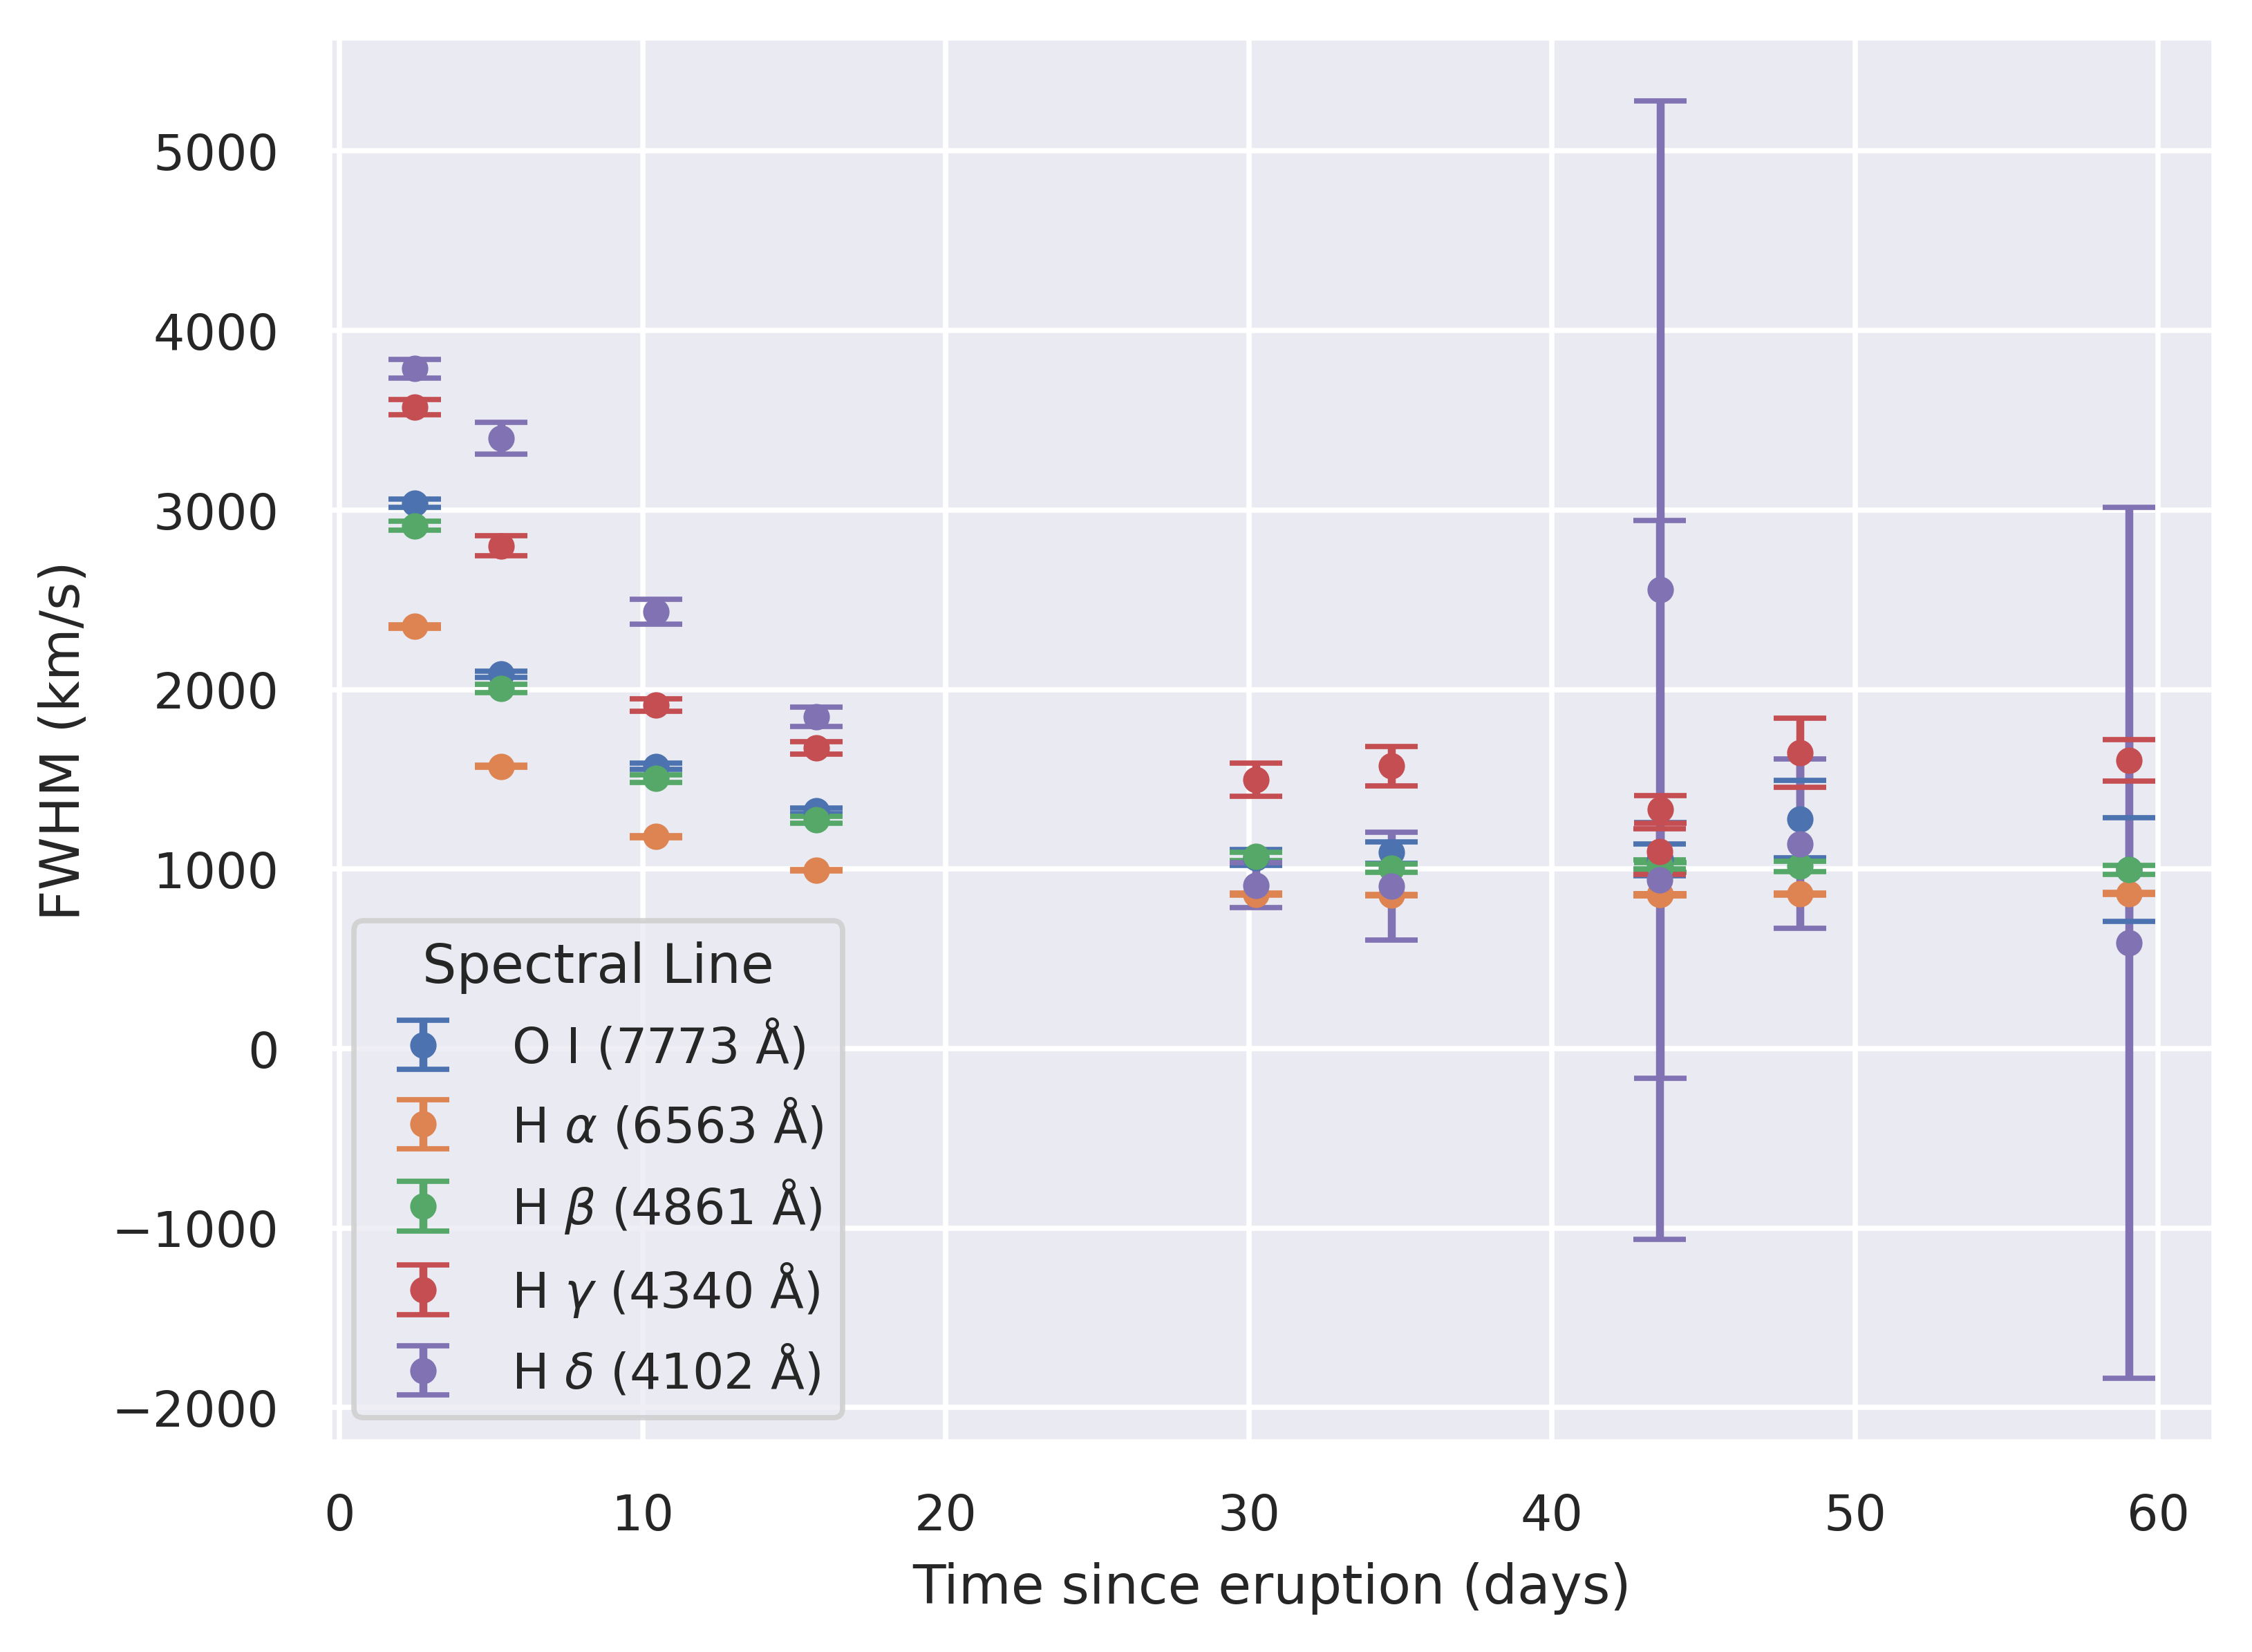
\includegraphics[width=\linewidth]{../codes/plots/line_width_evolution_kmps.png}
			\caption{Time evolution of FWHM (in units of km s\(^{-1}\)) of spectral lines.}
			\label{fig:line_width_evolution}
		\end{subfigure}
		\caption{Evolution of parameters derived from the analysis of spectroscopic images obtained over the course of \(\sim 60 days\).}
		\label{fig:time_evolution_parameters}
	\end{figure}

	In a similar manner, line fitting is performed for O \textsc{\romannumeral 1} (7773\r{A}) line and four Balmer lines, H \textsc{\(\delta\)} (4102\r{A}), H \textsc{\(\gamma\)} (4340\r{A}), H \textsc{\(\beta\)} (4861\r{A}) and H \textsc{\(\alpha\)} (6563\r{A}). The computed values of flux and full width half maximum (FWHM) are summarized in tables \ref{table:line_fluxes} and \ref{table:line_fwhm}, respectively. Although the values of FWHM are mentioned in units of wavelength change, \textit{i.e.} \r{A}, this is not the typical unit of representation. The values are often represented in units of velocity (km s\(^{-1}\)) because the span of a spectral line, quantified by FWHM is a function of velocity of the material emitting at the given wavelength. These units therefore help us understand the morphology and kinematics of the ejected material emitting at those wavelengths.

	The evolution of line fluxes, line flux ratios and line widths are shown in figures \ref{fig:line_flux_evolution}, \ref{fig:flux_ratio_evolution} and \ref{fig:line_width_evolution} respectively.


	If we plot the graphs in figure \ref{fig:time_evolution_parameters} on log-log plots, we can easily realise that all these evolutions can be described by simple power-law relations. As time evolves, nova ejecta is slowed down eventually as it reaches and collides with the circum-stellar material ejected by the star while it was still evolving. This slow down of velocity is evident from the time evolution of FWHM in units of velocity in figure \ref{fig:line_width_evolution}

	From the values of the ten employed continuum fits, it can be inferred that as the system evolves the overall value of the continuum across all wavelengths decreases. Continuum contribution in the blue wavelengths begins to dominate than in redder wavelengths as time evolves, and therefore, the colour of the nova tends towards blue as time evolves. Absolute magnitude value is estimated using photometry in section \ref{sec:photometry} and is of the order of \(\sim -8\) magnitudes. This is a fairly typical value for a classical nova.

	Using the equation,
	\[A_{r'} = 2.751 \times \textrm{E(B-V)}, \]
	we obtain a value of \(A_{r'} = 0.491 \pm 0.256\). This value can be used in equation \ref{eq:distance_modulus} to improve our estimate of distance of nova. Using equations \ref{eq:t2_mmrd}, \ref{eq:t3_mmrd} and \ref{eq:t15_mmrd}, we obtain the following distance estimates.
	\[d_{t_2} = 683.282^{+413.701}_{-257.683} \textrm{kpc,}\]
	\[d_{t_3} = 524.807^{+453.780}_{-243.358} \textrm{kpc,}\]
	\[d_{t_{15}} = 666.806^{+190.231}_{-148.006} \textrm{kpc.}\]
	Based on these distance estimates, The most probable location of the classical nova seems to be in M31 galaxy \citep{2012ApJ...745..156R}.

	\begin{thebibliography}{99}
		\bibitem[\protect\citeauthoryear{Poznanski et al.}{2012}]{na_abs_line}Dovi Poznanski, J. Xavier Prochaska, Joshua S. Bloom, An empirical relation between sodium absorption and dust extinction, Monthly Notices of the Royal Astronomical Society, Volume 426, Issue 2, 21 October 2012, Pages 1465–1474, https://doi.org/10.1111/j.1365-2966.2012.21796.x

		\bibitem[\protect\citeauthoryear{Strope, Schaefer, \& Henden}{2010}]{2010AJ....140...34S} Strope R.~J., Schaefer B.~E., Henden A.~A., 2010, AJ, 140, 34. doi:10.1088/0004-6256/140/1/34

		\bibitem[\protect\citeauthoryear{Tonry et al.}{2012}]{2012ApJ...750...99T} Tonry J.~L., Stubbs C.~W., Lykke K.~R., Doherty P., Shivvers I.~S., Burgett W.~S., Chambers K.~C., et al., 2012, ApJ, 750, 99. doi:10.1088/0004-637X/750/2/99

		\bibitem[\protect\citeauthoryear{Williams}{2012}]{2012AJ....144...98W} Williams R., 2012, AJ, 144, 98. doi:10.1088/0004-6256/144/4/98

		\bibitem[\protect\citeauthoryear{Downes \& Duerbeck}{2000}]{2000AJ....120.2007D} Downes R.~A., Duerbeck H.~W., 2000, AJ, 120, 2007. doi:10.1086/301551

		\bibitem[\protect\citeauthoryear{Darnley et al.}{2006}]{2006MNRAS.369..257D} Darnley M.~J., Bode M.~F., Kerins E., Newsam A.~M., An J., Baillon P., Belokurov V., et al., 2006, MNRAS, 369, 257. doi:10.1111/j.1365-2966.2006.10297.x

		\bibitem[\protect\citeauthoryear{Riess, Fliri, \& Valls-Gabaud}{2012}]{2012ApJ...745..156R} Riess A.~G., Fliri J., Valls-Gabaud D., 2012, ApJ, 745, 156. doi:10.1088/0004-637X/745/2/156

		\bibitem[\protect\citeauthoryear{Ferrarese, C{\^o}t{\'e}, \& Jord{\'a}n}{2003}]{2003ApJ...599.1302F} Ferrarese L., C{\^o}t{\'e} P., Jord{\'a}n A., 2003, ApJ, 599, 1302. doi:10.1086/379349

	\end{thebibliography}

	

\end{document}
